\documentclass{beamer}
\usepackage{epstopdf}
\usepackage{graphicx}
\usepackage{amsmath}
\setbeamerfont{caption}{series=\normalfont,size=\fontsize{4}{24}}

\title{Two-Qubit Dynamics with Josephson Qubits}
\author{John Meade \and Dylan Funk}
\date{April 2, 2015}

\begin{document}

\begin{frame}
\titlepage
\end{frame}

%%%%%%%%%%%%%%%%%%%%%%%%%%%%%%%%%%%%%%%%%%%%%%%%%%%%%%%%%%%%
% Background

\begin{frame}
    \vfill
    \centering
    \begin{beamercolorbox}[sep=8pt,center,shadow=true,rounded=true]{title}
        \usebeamerfont{title}
        Background
    \end{beamercolorbox}
    \vfill
\end{frame}

%%%

\begin{frame}
    \frametitle{Background}
    \framesubtitle{Cooper Pair Box}
    \begin{figure}[ht!]
        \centering
        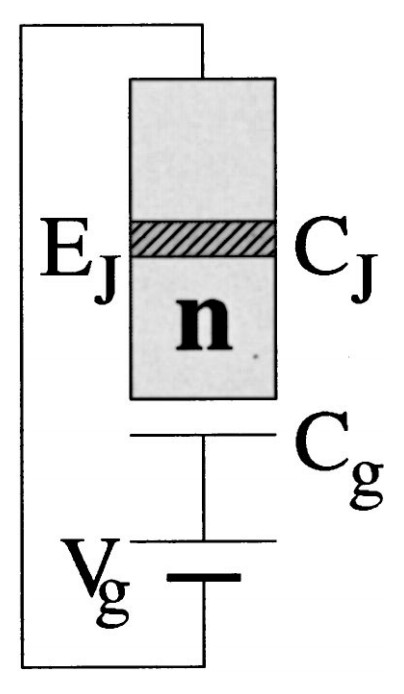
\includegraphics[height=0.6\textheight]{img/cooper-pair-box.jpg}
        \caption{http://journals.aps.org/rmp/pdf/10.1103/RevModPhys.73.357}
    \end{figure}
\end{frame}

%%%

\begin{frame}
    \frametitle{Background}
    \framesubtitle{SQUIDs}
    \begin{figure}[ht!]
        \centering
        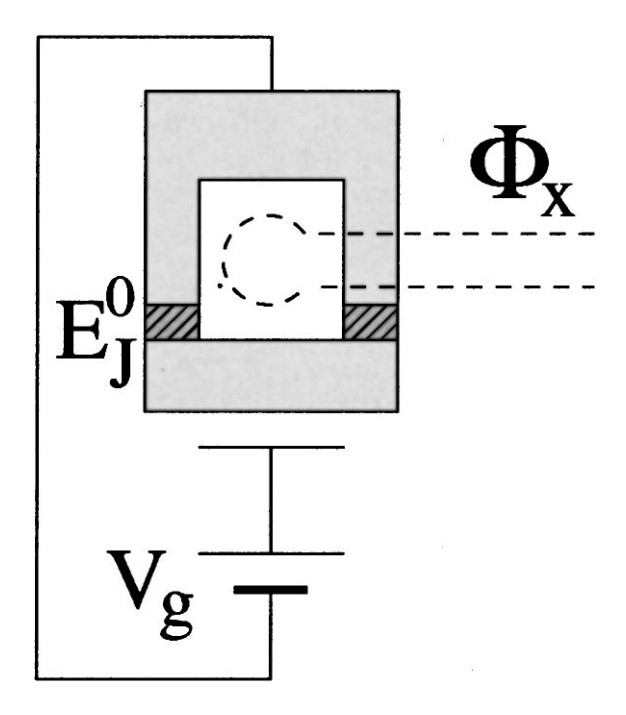
\includegraphics[height=0.6\textheight]{img/squid.jpg}
        \caption{http://journals.aps.org/rmp/pdf/10.1103/RevModPhys.73.357}
    \end{figure}
\end{frame}

%%%

\begin{frame}
    \frametitle{Background}
    \framesubtitle{Single-Qubit Charging Diagram}
    \begin{figure}[ht!]
        \centering
        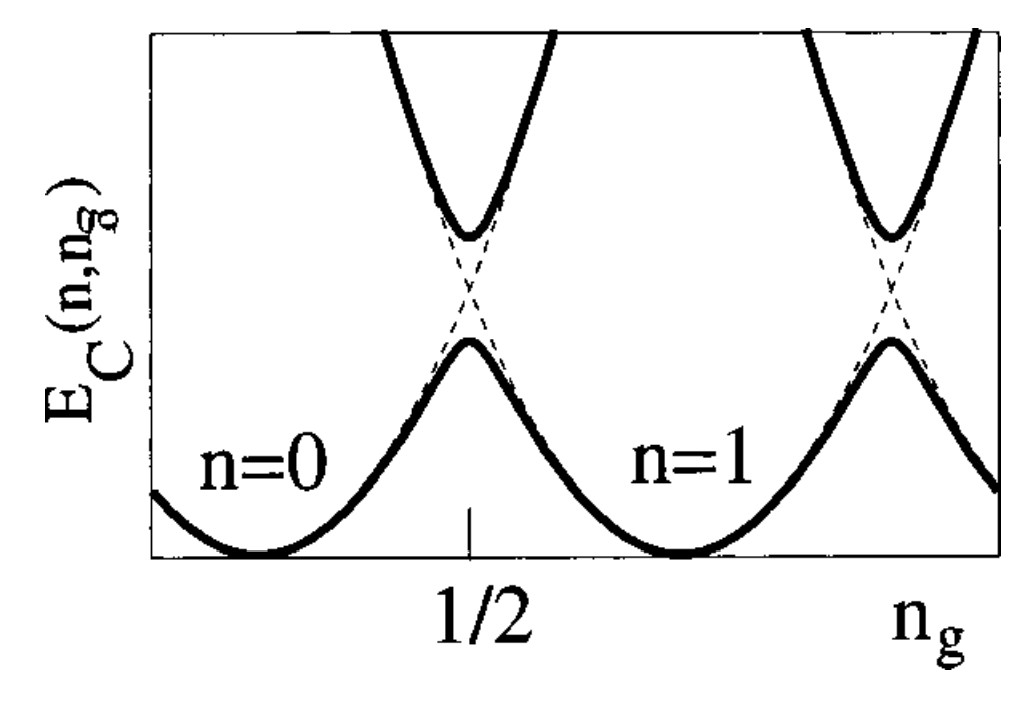
\includegraphics[width=0.8\textwidth]{img/single-qubit-band-diagram-only.jpg}
        \caption{A simple caption}
    \end{figure}
\end{frame}

%%%%%%%%%%%%%%%%%%%%%%%%%%%%%%%%%%%%%%%%%%%%%%%%%%%%%%%%%%%%
% Coupling of Two Qubits
% bulk of presentation here.
% should use 2-column layout often, to compare
% the one-qubit SQUID graphs to the graphs in the paper

\begin{frame}
    \vfill
    \centering
    \begin{beamercolorbox}[sep=8pt,center,shadow=true,rounded=true]{title}
        \usebeamerfont{title}
        Coupling of Two Qubits
    \end{beamercolorbox}
    \vfill
\end{frame}

%%%

\begin{frame}
    \frametitle{Coupling of Two Qubits}
    \framesubtitle{Basic Idea}
    \begin{figure}[!htb]
        \centering
        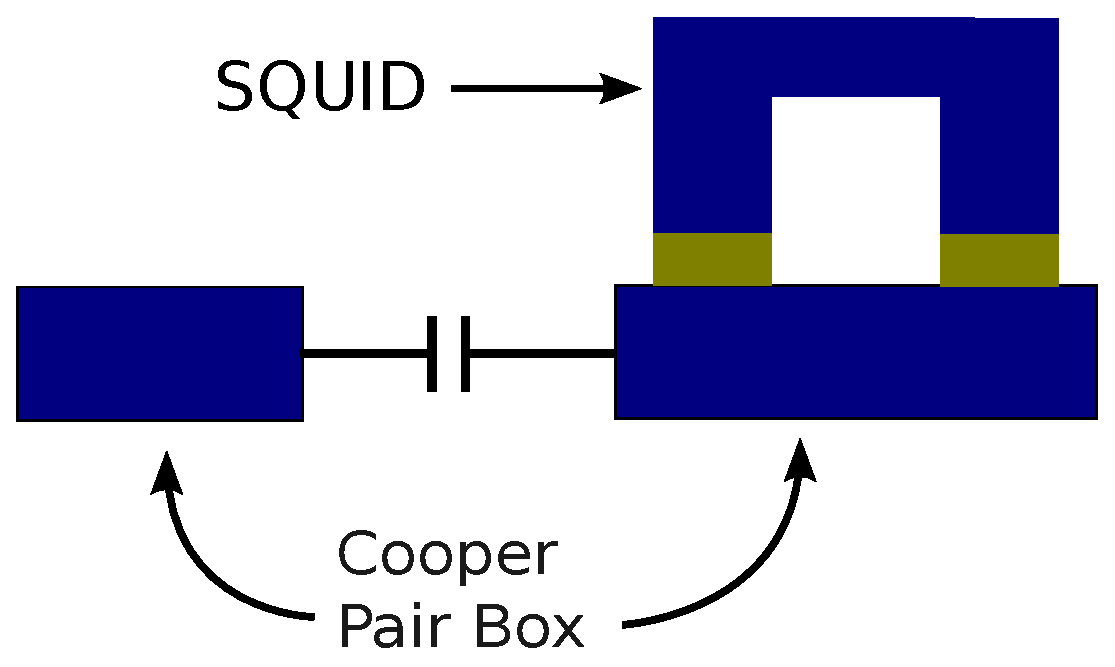
\includegraphics[width=0.8\textwidth]{img/basic-structure.eps}
    \end{figure}
\end{frame}

%%%

\begin{frame}
    \frametitle{Coupling of Two Qubits}
    \framesubtitle{The Circuit}
    \begin{figure}[ht!]
        \centering
        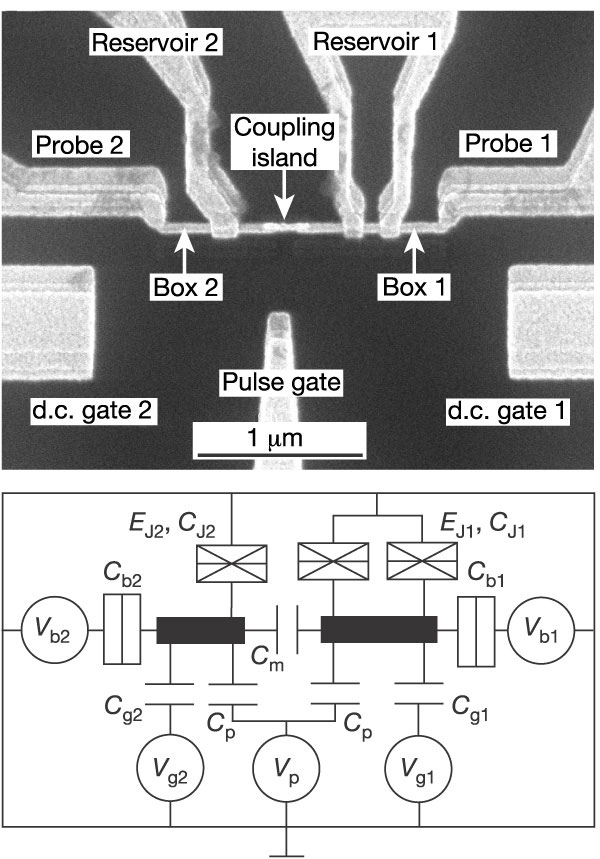
\includegraphics[height=0.7\textheight]{img/circuit-sem-and-diagram.jpg}
        \caption{http://www.nature.com/nature/journal/v421/n6925/full/nature01365.html}
    \end{figure}
\end{frame}

%%%

\begin{frame}
    \frametitle{Coupling of Two Qubits}
    \framesubtitle{Charging Diagram of Two-Qubit Case}
    \begin{figure}[ht!]
        \centering
        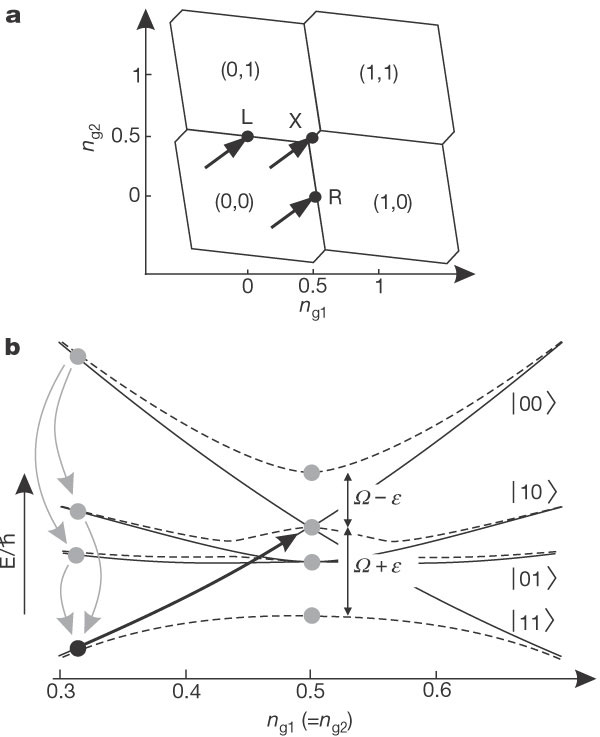
\includegraphics[height=0.6\textheight]{img/charging-diagram.jpg}
        \caption{http://www.nature.com/nature/journal/v421/n6925/full/nature01365.html}
    \end{figure}
\end{frame}

%%%

\begin{frame}
    \frametitle{Coupling of Two Qubits}
    \framesubtitle{Points L and R}
    \begin{figure}[ht!]
        \centering
        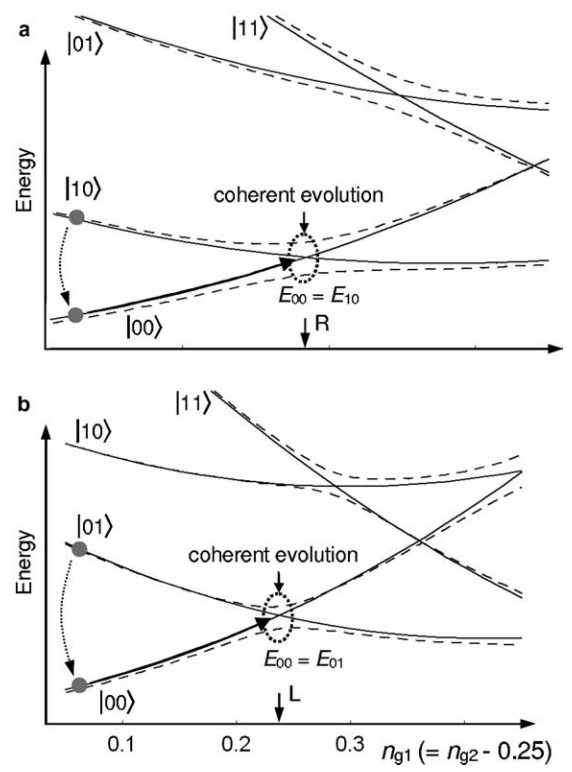
\includegraphics[height=0.6\textheight]{img/points-l-and-r.jpg}
        \caption{http://citeseerx.ist.psu.edu/viewdoc/download?doi=10.1.1.193.5098\&rep=rep1\&type=pdf}
    \end{figure}
\end{frame}

%%%

\begin{frame}
    \frametitle{Coupling of Two Qubits}
    \framesubtitle{Charging Diagram Level Curves}
    \begin{figure}[ht!]
        \centering
        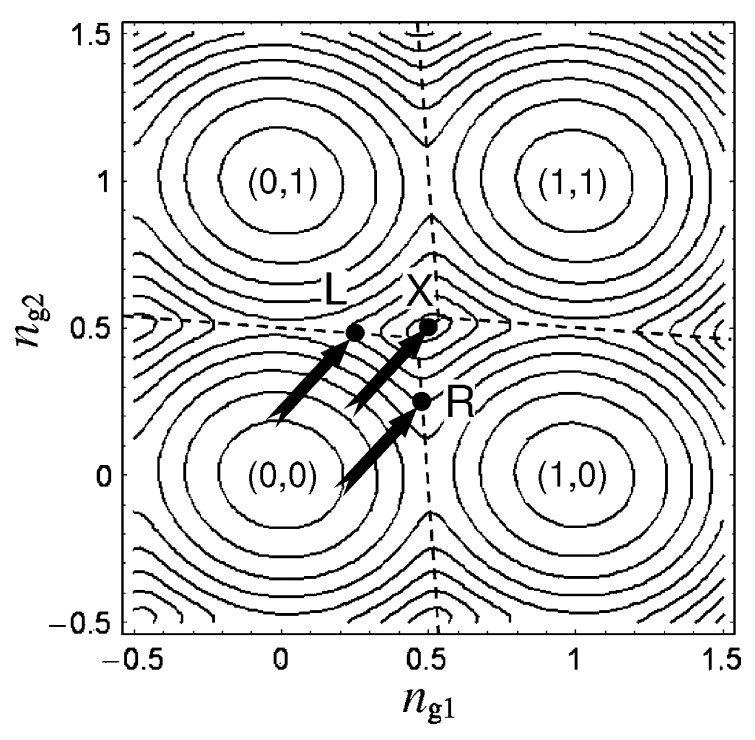
\includegraphics[height=0.6\textheight]{img/charging-level-curves.jpg}
        \caption{http://citeseerx.ist.psu.edu/viewdoc/download?doi=10.1.1.193.5098\&rep=rep1\&type=pdf}
    \end{figure}
\end{frame}

%%%

\begin{frame}
    \frametitle{Coupling of Two Qubits}
    \framesubtitle{Charging-Energy Diagram}
    \begin{figure}[ht!]
        \centering
        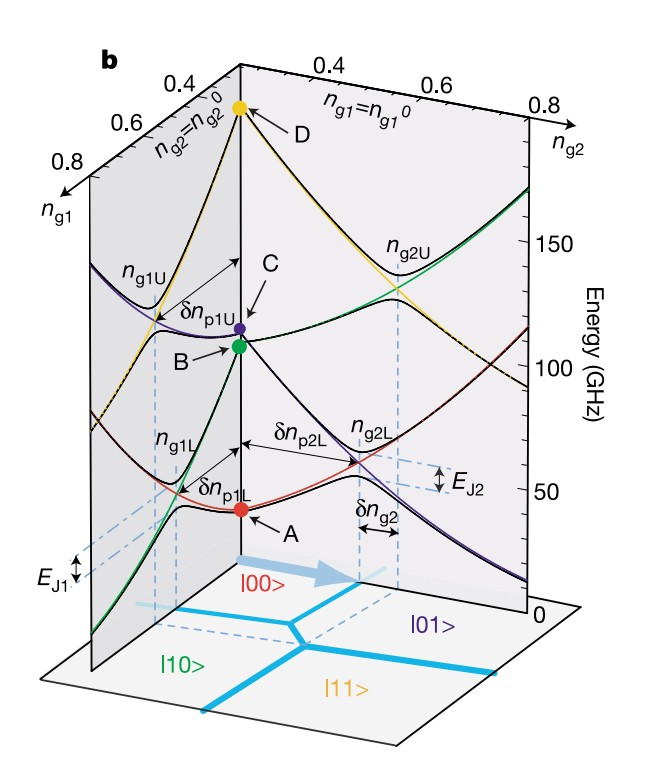
\includegraphics[height=0.6\textheight]{img/charging-energy-diagram.jpg}
        \caption{http://qudev.ethz.ch/content/courses/QSIT09/pdfs/Yamamoto2003.pdf}
    \end{figure}
\end{frame}

%%%

\begin{frame}
    \frametitle{Coupling of Two Qubits}
    \framesubtitle{Theory}
    \begin{block}{Hamiltonian}
        \fontsize{8}{7.2}\selectfont
        $$
        H=
        \begingroup
            \renewcommand*{\arraystretch}{1.5}
            \begin{bmatrix}
                E_{00} & -\frac{1}{2}E_{J1} & -\frac{1}{2}E_{J2} & 0 \\
                -\frac{1}{2}E_{J1} & E_{10} & 0 & -\frac{1}{2}E_{J2} \\
                -\frac{1}{2}E_{J2} & 0 & E_{01} & -\frac{1}{2}E_{J1} \\
                0 & -\frac{1}{2}E_{J2} & -\frac{1}{2}E_{J1} & E_{11}
            \end{bmatrix}
        \endgroup
        $$
        
        Where...
        \begin{itemize}
            \item $E_{n1n2}=E_{c1}(n_{g1}-n_1)^2 + E_{c2}(n_{g2}-n_2)^2 + E_{m}(n_{g1}-n_1)(n_{g2}-n_2)$
            \item $E_{Ji}$ is the Josephson energy of the $i^{th}$ box
            \item $E_{c1,c2}=4e^2C_{\Sigma 2,\Sigma 1} / 2(C_{\Sigma 1} C_{\Sigma 2} - C_m^2)$ are the effective Cooper pair charging energies
            \item $C_{\Sigma i}$ is the sum of all capacitances connected to the $i^{th}$ island
            \item $n_{g1,g2}=(C_{g1,g2}V_{g1,g2}+C_pV_p)/2e$ is the charge, indiced by the gate and pulse voltages, on the qubits
            \item $E_m=4e^2C_m/(C_{\Sigma 1}C_{\Sigma 2}-C_m^2)$ is the coupling energy of the qubits
        \end{itemize}
    \end{block}
\end{frame}

%%%

\begin{frame}
    \frametitle{Coupling of Two Qubits}
    \framesubtitle{Theory}
    \begin{block}{Probabilities}
        \fontsize{8}{14}\selectfont
        \begin{itemize}
            \item At the coresonance point, we have a coherent superposition state $|\psi\rangle=c_1|00\rangle + c_2|10\rangle + c_3|01\rangle + c_4|11\rangle$

            \item ie, the qubit state probabilities are $p_1(1) = |c_2|^2 + |c_4|^2$ and $p_2(1) = |c_3|^2 + |c_4|^2$

            \item Now we initialize system to $|\psi\rangle=|00\rangle$

            \item Using this Hamiltonian and an ideal rectangular pulse of length $\Delta t$, $p_{1,2}(1)=\frac{1}{4} \Bigg ( 2-(1-\chi_{1,2})cos[(\Omega+\epsilon)\Delta t]-(1+\chi_{1,2})cos[(\Omega-\epsilon)\Delta t] \Bigg )$

            Where...
            \begin{itemize}
                \item $\chi_{1,2}=\frac{(E^2_{J2,J1}-E^2_{J1,J2})+E^2_m/4}{4\hbar^2\Omega\epsilon}$
                \item $\Omega = \sqrt{(E_{J1}+E_{J2})^2+(E_m/2)^2}/2\hbar$
                \item $\epsilon = \sqrt{(E_{J1}-E_{J2})^2+(E_m/2)^2}/2\hbar$
            \end{itemize}
        \end{itemize}
    \end{block}
\end{frame}

%%%

\begin{frame}
    \frametitle{Coupling of Two Qubits}
    \framesubtitle{State Readout}
    \begin{figure}[!htb]
        \centering
        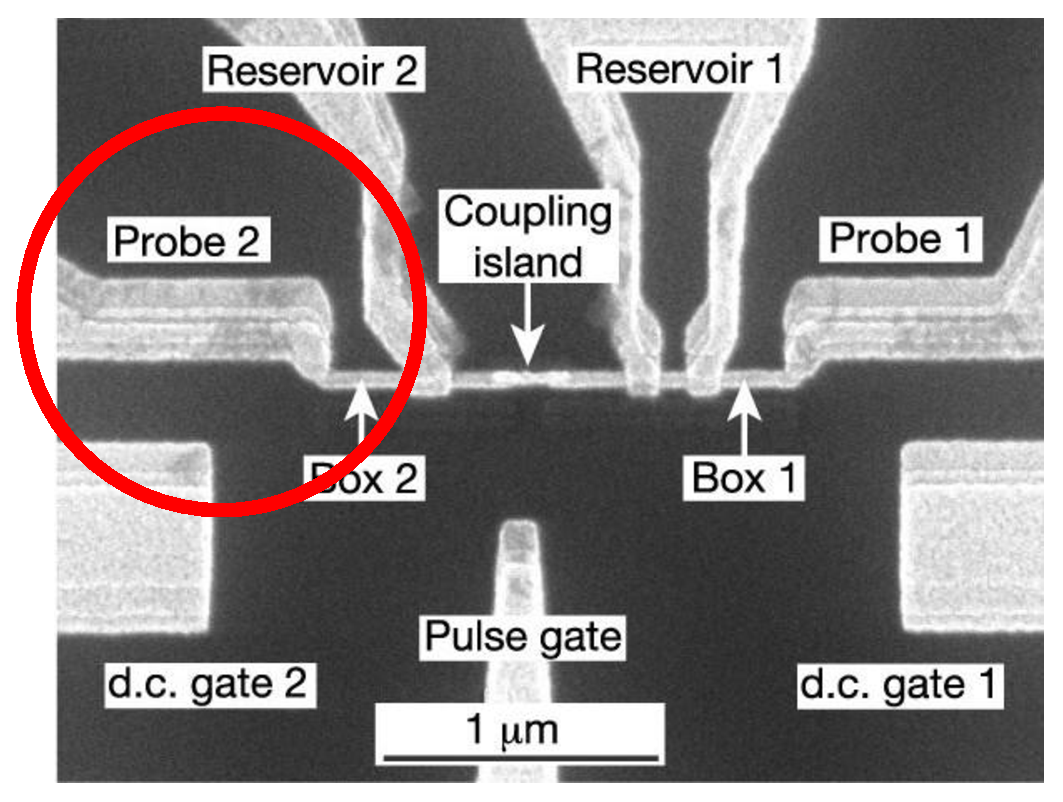
\includegraphics[width=0.8\textwidth]{img/two-qubit-sem-probe.eps}
        \caption{http://www.nature.com/nature/journal/v421/n6925/full/nature01365.html}
    \end{figure}
\end{frame}

%%%

\begin{frame}
    \frametitle{Coupling of Two Qubits}
    \framesubtitle{Parameter Measurements / Frequency Responses}
    \begin{columns}
        \column{.35\textwidth}
            \fontsize{6}{9}\selectfont
            Probe currents are proportional to the qubit state probabilities: $I_1 \propto p_1(1) = |c_2|^2 + |c_4|^2$ and $I_2 \propto p_2(1) = |c_3|^2 + |c_4|^2$
            \begin{itemize}
                \item Tune system by bringing to point L or R, exciting oscillations in one qubit
                \item Get cosines with exponential decay
                \item Fourier transform gives frequencies, which define $E_{J1}$ or $E_{J2}$
                \item Drive system to point X and perform same Fourier measurement
                \item This time, get 2 frequencies, $\Omega \pm \epsilon$
            \end{itemize}
        \column{.65\textwidth}
            \begin{figure}[ht!]
                \centering
                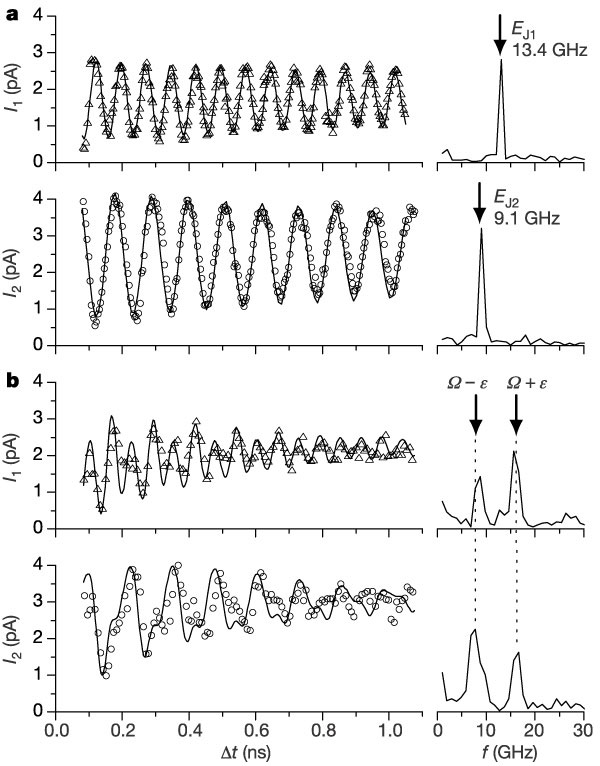
\includegraphics[height=0.6\textheight]{img/probe-current-osc.jpg}
                \caption{http://www.nature.com/nature/journal/v421/n6925/full/nature01365.html}
            \end{figure}
    \end{columns}
\end{frame}

%%%

\begin{frame}
    \frametitle{Coupling of Two Qubits}
    \framesubtitle{EJ1 dependence of spectrum components}
    \begin{block}{}
        \centering
        Note: Frequency repulsion at $E_{J1} \approx E_{J2}$
    \end{block}
    \begin{figure}[ht!]
        \centering
        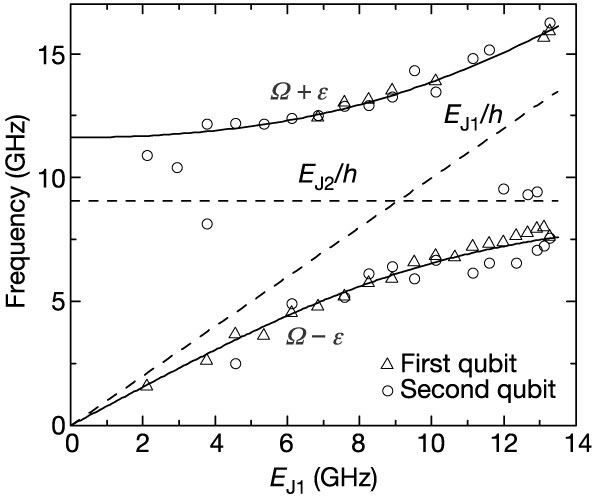
\includegraphics[height=0.6\textheight]{img/freq-vs-ej1.jpg}
        \caption{http://www.nature.com/nature/journal/v421/n6925/full/nature01365.html}
    \end{figure}
\end{frame}

%%%

\begin{frame}
    \frametitle{Coupling of Two Qubits}
    \framesubtitle{Decoherence}
    \centering
    \begin{itemize}
        \item Probe Junction
        \item Charge Qubit Noise, ie $n_g \rightarrow n_g + \delta n_g(t)$
        \item Solid State Noise
        \begin{itemize}
            \item Thermal Noise
            \item Material Imperfections
            \item Charge and Flux Noise
        \end{itemize}
    \end{itemize}
\end{frame}

%%%%%%%%%%%%%%%%%%%%%%%%%%%%%%%%%%%%%%%%%%%%%%%%%%%%%%%%%%%%
% Fabrication Techniques

\begin{frame}
    \vfill
    \centering
    \begin{beamercolorbox}[sep=8pt,center,shadow=true,rounded=true]{title}
        \usebeamerfont{title}
        Fabrication Techniques
    \end{beamercolorbox}
    \vfill
\end{frame}

%%%

\begin{frame}
    \frametitle{Fabrication Techniques}
    \framesubtitle{Evapouration (Deposition)}
    \begin{figure}[!htb]
        \centering
        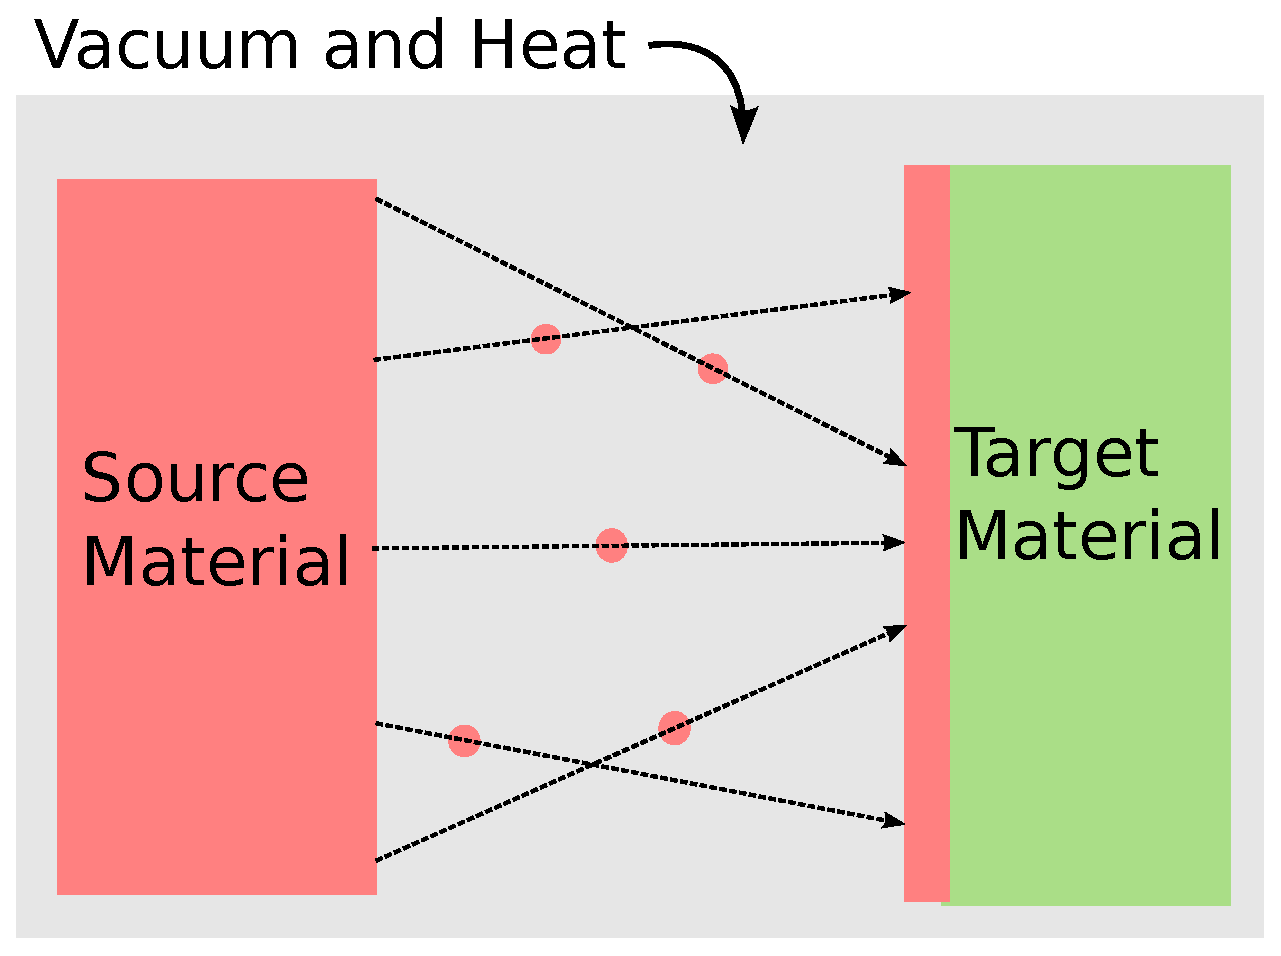
\includegraphics[width=0.8\textwidth]{img/evaporation.eps}
    \end{figure}
\end{frame}

%%%

\begin{frame}
    \frametitle{Fabrication Techniques}
    \framesubtitle{Shadow Evapouration}
    \begin{figure}[ht!]
        \centering
        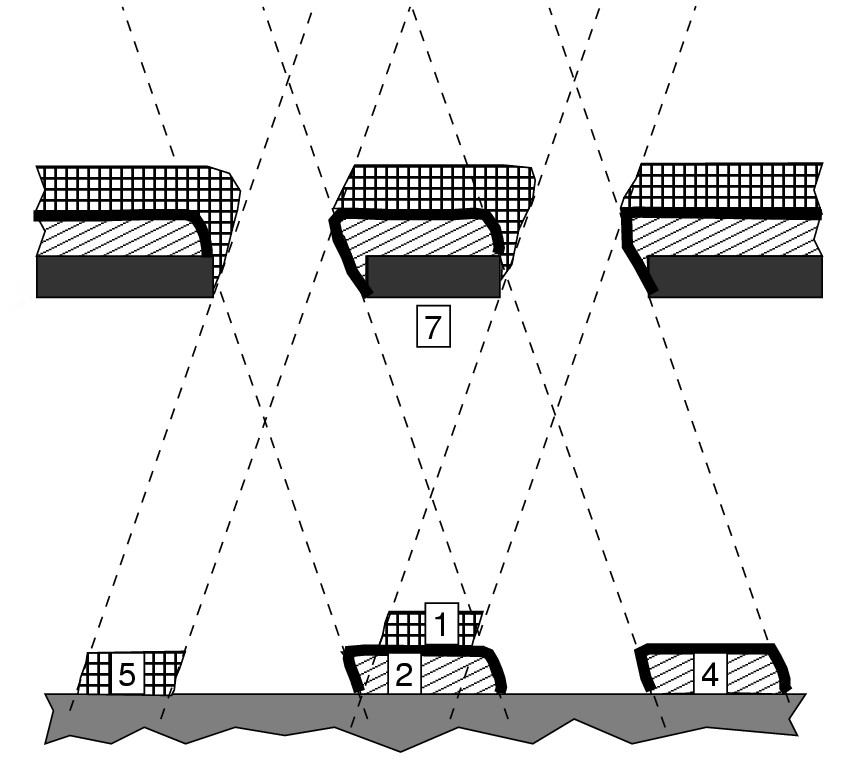
\includegraphics[width=0.7\textwidth]{img/shadow-evaporation.png}
        \caption{http://en.wikipedia.org/wiki/Niemeyer-Dolan\_technique}
    \end{figure}
\end{frame}

%%%

\begin{frame}
    \frametitle{Fabrication Techniques}
    \framesubtitle{Electron Beam Lithography (EBL)}
    \begin{figure}[!htb]
        \centering
        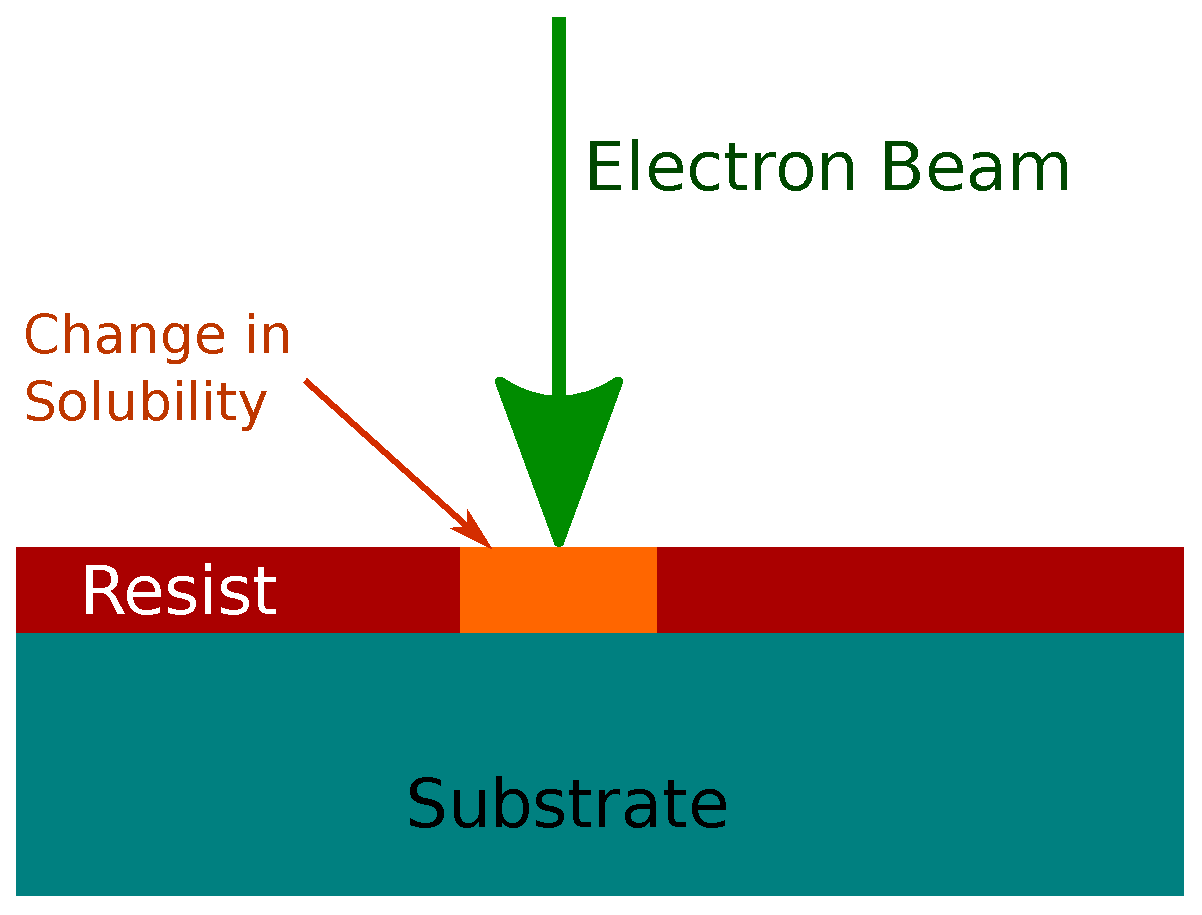
\includegraphics[height=0.8\textheight]{img/ebeam.eps}
    \end{figure}
\end{frame}

%%%

\begin{frame}
    \frametitle{Fabrication Techniques}
    \framesubtitle{Etching}
    \begin{figure}[ht!]
        \centering
        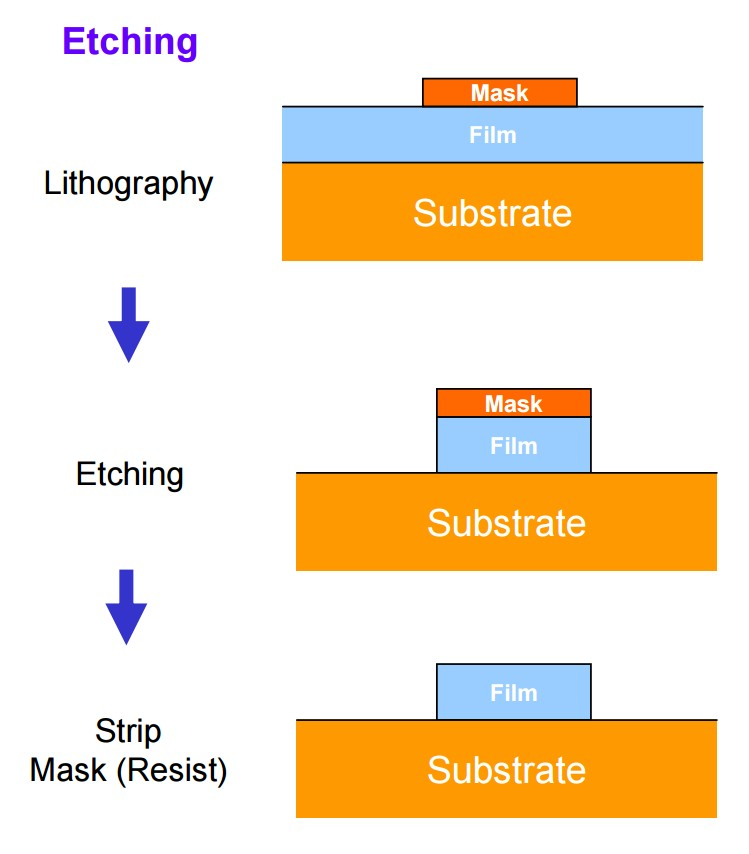
\includegraphics[height=0.6\textheight]{img/etching.jpg}
        \caption[10pt]{http://www.mrsec.harvard.edu/education/ap298r2004/Erli\%20chen\%20Fabrication\%20III\%20-\%20Etching.pdf}
    \end{figure}
\end{frame}

%%%

\begin{frame}
    \frametitle{Fabrication Techniques}
    \framesubtitle{Lift-off}
    \begin{figure}[!htb]
        \centering
        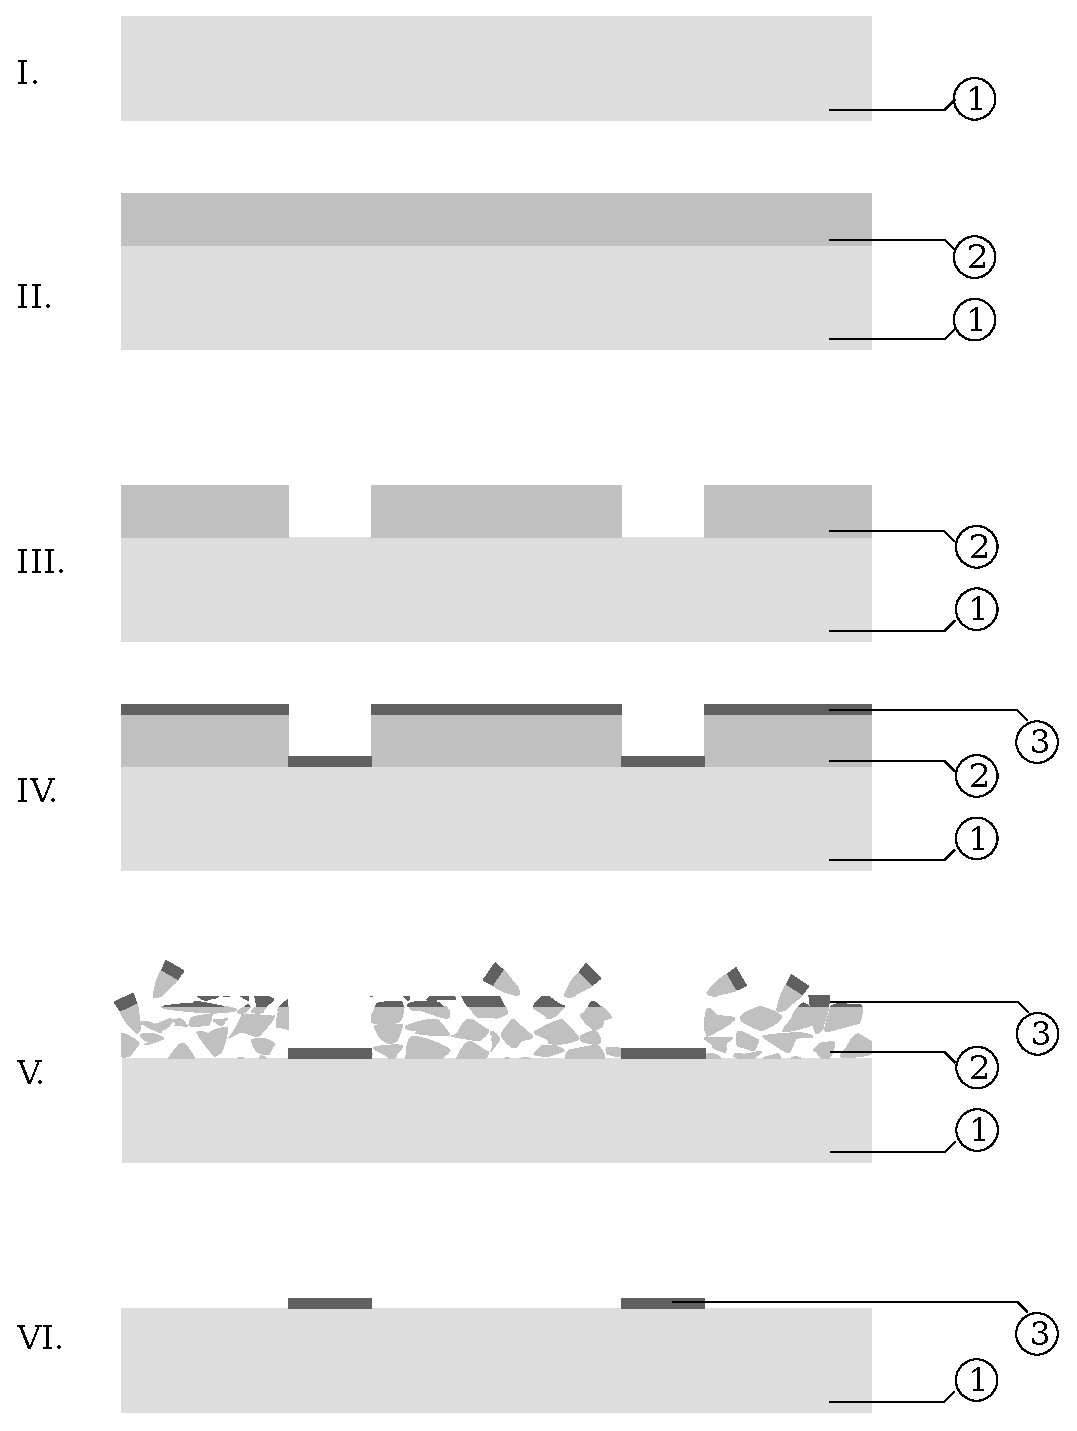
\includegraphics[height=0.6\textheight]{img/lift-off.eps}
        \caption{http://en.wikipedia.org/wiki/Lift-off\_\%28microtechnology\%29}
    \end{figure}
\end{frame}

%%%

\begin{frame}
    \frametitle{Fabrication Techniques}
    \framesubtitle{SEM image of a SQUID qubit}
    \begin{figure}[ht!]
        \centering
        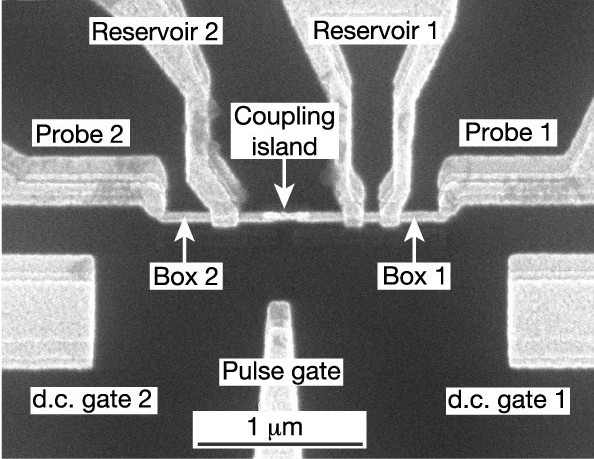
\includegraphics[width=0.7\textwidth]{img/two-qubit-sem.jpg}
        \caption{http://www.nature.com/nature/journal/v421/n6925/full/nature01365.html}
    \end{figure}
\end{frame}

%%%%%%%%%%%%%%%%%%%%%%%%%%%%%%%%%%%%%%%%%%%%%%%%%%%%%%%%%%%%

\begin{frame}
    \frametitle{THE END}
    \framesubtitle{THE END}
    \begin{block}{}
        \begin{columns}
            \column{.5\textwidth}
                \begin{block}{THE END}
                    THE END
                \end{block}
            \column{.5\textwidth}
                \begin{block}{THE END}
                    \begin{itemize}
                        \item THE END
                        \item THE END
                        \item THE END
                        \item THE END.
                    \end{itemize}
                \end{block}
        \end{columns}
    \end{block}
    \begin{block}{Reference Papers}
        \fontsize{6}{7.2}\selectfont
        http://www.nature.com/nature/journal/v421/n6925/full/nature01365.html

        http://citeseerx.ist.psu.edu/viewdoc/download?doi=10.1.1.193.5098\&rep=rep1\&type=pdf

        (Figures cited individually)
    \end{block}
\end{frame}

\end{document}
